\chapter{Methodology}%    \chapter{}  = level 1, top level


	\section{Problem Definition}
		The main challenge for optimizing container yard operations at the Ports of Auckland was predicting dwell times
		to support placement decisions.
		\\
		\\
		Predicting the exact number of days for each container was the first approach. Using classifier models with the
		selected features, predicting how many days each container would stay in the port was set as a target. The
		metrics in the models, especially accuracy, were low.
		\\
		\\
		The variance in the predicted days was tremendous. Some similar-character containers were taken out daily while
		others stuck around for weeks. There needed to be a clear pattern for the classifier to generate acceptable
		predictions.
		\\
		\\
		Rather than predicting an exact number of days, a range of days was a better approach improving the results.
		Having more than one range of days allows port managers to have options to make decisions, balancing prediction
		accuracy with operational utility.


	\section{Dataset Strategy and Model Evaluation}

		The experimental approach employs a temporal split strategy to ensure robust model development and realistic
		performance evaluation. As detailed in Table~\ref{tab:dataset-split}
		, 2023 dataset will be used for the development phase, allocating 80\% for training and 20\%
		for cross-validation. This split enables thorough model tuning and hyperparameter optimization while
		maintaining statistical validity. For final evaluation, 2024 dataset will be used as an unseen test
		set, providing a true assessment of how the models perform on future data. This temporal separation is
		crucial as it mirrors real-world conditions where models must predict outcomes for future periods.

		\begin{table}[ht]
			\centering
			\begin{tabular}{|l|c|l|}
				\hline
				\textbf{Time Period} & \textbf{Data Split} & \textbf{Purpose}                             \\
				\hline
				\multirow{2023}          & 80\%                & Training Set: Model development and fitting  \\
				& 20\%                & Validation Set: Cross-validation and tuning  \\
				\hline
				2024                     & 100\%               & Testing Set: Final evaluation on unseen data \\
				\hline
			\end{tabular}
			\caption{Dataset Split Strategy for Model Development and Evaluation}
			\label{tab:dataset-split}
		\end{table}

		The development process begins with initial model training on the 2023 training set. Cross-validation
		techniques are employed during this phase to optimize model hyperparameters and assess performance
		stability. Once the bet models are selected and tuned, those final models will be evaluated over the 2024
		dataset. This approach provides a rigorous test of model generalization, as the evaluation data represents
		genuinely unseen future observations.


	\section{Selecting Time Range Categories and Classifiers}
		This research took a data-driven approach to identify an optimal set of ranges of days to predict dwell time.
		Iteratively, multiple time range configurations were tested to find groupings that allowed operational needs to
		be achieved and predictions with solid performance generated.
		\\
		\\
		The search for optimal time ranges involved systematically evaluating different bin configurations. Each
		configuration was tested across multiple machine learning algorithms to ensure the selected ranges would be
		robust across different modeling approaches. The goal was to find time ranges reflecting meaningful operational
		distinctions in container handling, provide sufficient data in each category for reliable model training, and
		enable predictive solid performance across different algorithms.
		\\
		\\
		Multiple models were fit, using the training set (table~\ref{tab:dataset-split}
		), to be evaluated based on their metrics in finding ranges of days and classifiers. The models and ranges
		with the best performance, evaluated by F1 Score, were chosen to follow the next step: prediction evaluation.
		\\
		\\
		Five classifiers were fitted initially: Random Forest, K-Nearest Neighbors, Logistic Regression, Gradient
		Boosting, and Naive Bayes (table~\ref{tab:model-type-counts}).

		\begin{table}[ht]
			\centering
			\begin{tabular}{|l|c|}
				\hline
				\textbf{Model Type} & \textbf{Models Fitted} \\
				\hline
				Gradient Boosting       & 64                     \\
				KNN                     & 64                     \\
				Logistic Regression     & 64                     \\
				Naïve Bayes             & 52                     \\
				Random Forest           & 64                     \\
				\hline
				\textbf{Grand Total}    & \textbf{308}           \\
				\hline
			\end{tabular}
			\caption{Number of Models Fitted by Type}
			\label{tab:model-type-counts}
		\end{table}

		Random Forest was a top performer (Table~\ref{tab:model-type-performance}) with an impressive 87.0\%
		F1 Score, showing remarkable consistency with its similar accuracy of 86.9\%
		, having the best overall balance between precision and recall.
		KNN's performance had the second place with 86.0\%
		F1 Score close to Random Forest in both metrics. More powerful classifier than initially expected.
		Gradient Boosting and Logistic Regression performed adequately but notably below the top two. Gradient
		Boosting achieved 77.0\% F1 Score while Logistic Regression close behind at 76.0\%
		. Naïve Bayes underperformed with just a 5.0\%
		F1 Score, clearly not suitable for this specific prediction task.

		\begin{table}[ht]
			\centering
			\begin{tabular}{|l|c|c|}
				\hline
				\textbf{Model Type} & \textbf{Max F1 Score} & \textbf{Max Test Accuracy} \\
				\hline
				Random Forest           & 87.0\%                & 86.9\%                     \\
				KNN                     & 86.0\%                & 86.3\%                     \\
				Gradient Boosting       & 77.0\%                & 78.7\%                     \\
				Logistic Regression     & 76.0\%                & 76.7\%                     \\
				Naïve Bayes             & 5.0\%                 & 9.6\%                      \\
				\hline
			\end{tabular}
			\caption{Model Type Performance Metrics}
			\label{tab:model-type-performance}
		\end{table}

		The models selected with appropriate metrics were Random Forest, KNN, Gradient Boosting and Logistic
		Regression.

		After being sure that there were models that performed as expected, the next step was selecting the
		group of range to be used in the model. Those models were fitted with multiple groups of ranges to allow a
		posterior analysis based on F1-Score values, making sure that at least any range was significant.

		\subsection{Finding Ranges and Defining data scaling strategy}

			Some groups of ranges were over 80\% (table~\ref{tab:bins-ranges})
			of accuracy and F1-Score. As there were appropriate thresholds of metrics overtaken, the analysis
			continued over classifiers to check which ranges were shared among them. The best ones were kept for
			posterior analysis.

			\begin{table}[ht]
				\centering
				\small
				\begin{tabular}{|l|c|c|c|}
					\hline
					\textbf{Bins Ranges} & \textbf{Models Fitted} & \textbf{Max Test Accuracy}
					& \textbf{Max F1 Score}
					\\
					\hline
					{[}0, 3, 10, 21{]} & 20 & 79\% & 79.0\% \\
					{[}0, 3, 11, 21{]} & 20 & 80\% & 80.0\% \\
					{[}0, 3, 12, 21{]} & 20 & 80\% & 80.0\% \\
					{[}0, 3, 9, 21{]}  & 20 & 78\% & 77.0\% \\
					{[}0, 4, 10, 21{]} & 16 & 83\% & 82.0\% \\
					{[}0, 4, 11, 21{]} & 16 & 83\% & 83.0\% \\
					{[}0, 4, 12, 21{]} & 20 & 84\% & 83.0\% \\
					{[}0, 4, 9, 21{]}  & 16 & 81\% & 81.0\% \\
					{[}0, 5, 10, 21{]} & 20 & 85\% & 85.0\% \\
					{[}0, 5, 11, 21{]} & 20 & 85\% & 85.0\% \\
					{[}0, 5, 12, 21{]} & 20 & 86\% & 85.0\% \\
					{[}0, 5, 9, 21{]}  & 20 & 84\% & 84.0\% \\
					{[}0, 6, 10, 21{]} & 20 & 86\% & 86.0\% \\
					{[}0, 6, 11, 21{]} & 20 & 87\% & 86.0\% \\
					{[}0, 6, 12, 21{]} & 20 & 87\% & 87.0\% \\
					{[}0, 6, 9, 21{]} & 20 & 86\% & 85.0\%
					\\
					\hline
					\textbf{Total} & \textbf{308} & \textbf{} & \textbf{}
					\\
					\hline
				\end{tabular}
				\caption{Ranges and Max possible F1-Scores and accuracy by Fitted Models}
				\label{tab:bins-ranges}
			\end{table}

			Additionally, each model and range was also trained using a combination of techniques, including
			scaling via SMOTE (Synthetic Minority Over-sampling Technique) and stratification based on weekly and
			monthly. The goal was to explore whether scaling or stratification would improve the model’s ability to
			handle imbalanced data effectively.

			\begin{table}[ht]
				\centering
				\small
				\begin{tabular}{|l|c|c|c|c|c|}
					\hline
					\textbf{Range} & \textbf{F1 Score} & \textbf{Precision} & \textbf{Recall} & \textbf{Scaled}
					& \textbf{Stratified}
					\\
					\hline
					\multicolumn{6}{|l|}{\textbf{[0, 4, 10, 21]}} \\
					\hline
					& 0.81 & 0.81 & 0.81 & False & False \\
					& 0.81 & 0.81 & 0.81 & False & True  \\
					& 0.81 & 0.81 & 0.81 & True  & False \\
					& 0.81 & 0.81 & 0.81 & True  & True  \\
					& 0.81 & 0.82 & 0.81 & True  & False \\
					& 0.82 & 0.82 & 0.83 & False & False \\
					& 0.82 & 0.83 & 0.83 & False & True  \\
					\hline
					\multicolumn{6}{|l|}{\textbf{[0, 4, 11, 21]}} \\
					\hline
					& 0.81 & 0.82 & 0.82 & True  & True  \\
					& 0.82 & 0.82 & 0.82 & False & False \\
					& 0.82 & 0.82 & 0.82 & False & True  \\
					& 0.82 & 0.82 & 0.82 & True  & False \\
					& 0.82 & 0.83 & 0.82 & True  & False \\
					& 0.83 & 0.83 & 0.83 & False & False \\
					& 0.83 & 0.83 & 0.83 & False & True  \\
					\hline
					\multicolumn{6}{|l|}{\textbf{[0, 4, 12, 21]}} \\
					\hline
					& 0.81 & 0.82 & 0.80 & True  & True  \\
					& 0.82 & 0.82 & 0.82 & False & False \\
					& 0.82 & 0.82 & 0.82 & False & True  \\
					& 0.82 & 0.82 & 0.82 & True  & False \\
					& 0.82 & 0.82 & 0.82 & True  & True  \\
					& 0.83 & 0.83 & 0.82 & True  & False \\
					& 0.83 & 0.84 & 0.84 & False & False \\
					& 0.83 & 0.84 & 0.84 & False & True  \\
					\hline
				\end{tabular}
				\caption{Performance Metrics by Range Under Different Conditions}
				\label{tab:bins-performance-conditions}
			\end{table}


			After multiple iterations and testing (table~\ref{tab:bins-performance-conditions}
			), regarding data scaling and stratification, the metrics in each approach did not lead to any significant
			improvements and, in some cases, resulted in worse performance. Consequently, it was determined that
			neither scaling nor stratification was beneficial for this particular dataset, and these techniques
			were not applied in the final model.
			\\
			\\
			Given the presence of attractive ranges and classifiers and the fact that no stratification or scaling was
			required, a group of ranges was selected. The optimal group, identified as the best across all the
			configurations, consisted of 0-3 days, 4-11 days, and 12+ days ([0, 4, 12, 21]). These groups of ranges
			provided solid performance, an acceptable data distribution (fig. \ref{fig:class_ranges_distribution}
			) while allowing the defined ranges to be good enough to establish stacking strategies for the
			port.

			\begin{figure}[ht]
				\centering
				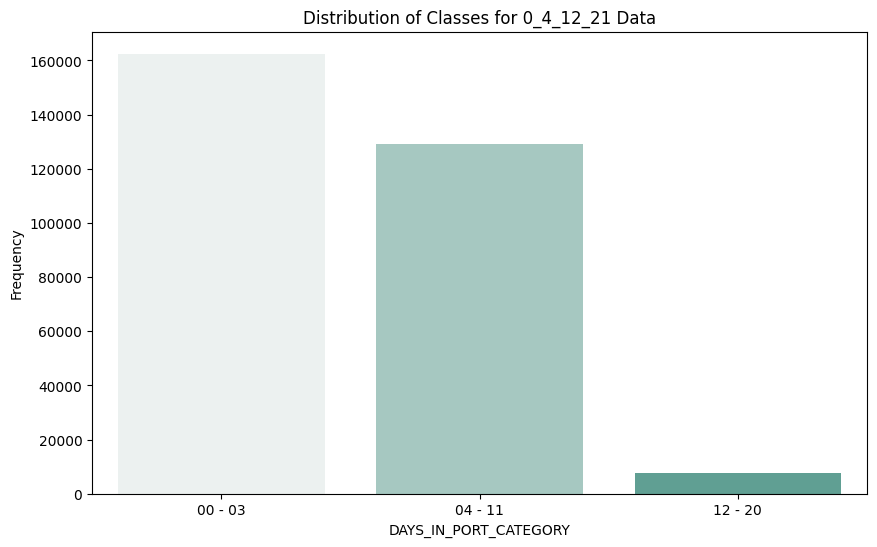
\includegraphics[width=0.5\textwidth]{images/ClassRangesDistribution}
				\caption{Ranges Distribution Labels}
				\label{fig:class_ranges_distribution}
			\end{figure}

		\subsection{Class Imbalance Analysis}

			The distribution of container dwell times are imbalanced across the three categories (fig.~
			\ref{fig:class_ranges_distribution}
			). The largest group, the short-term stays (0-3 days), has around 160,000 containers. For
			Medium-term stays (4-11 days), there are about 130,000 containers. For the smallest group, long-term
			stays (12-20 days), there are significantly fewer containers, with only 10,000 units representing a small
			portion of the overall data.

		\subsection{Selecting the Metric: F1 Score}

			\subsubsection{Addressing the Imbalance:}
				Ranges evaluated were more common than others (Figure~
				\ref{fig:class_ranges_distribution}
				), which led to an imbalanced evaluation, generating a wrong sense of good predictions. The accuracy
				metric misled these models' results by predicting the most frequent classes. F1-Score corrected this,
				providing a more appropriate understanding of the real performance.
				\\
				\\
				Due to this imbalanced distribution, the F1 Score provides a handy evaluation metric. Since accuracy
				could be misleading, with short and medium-term stays making up more than 95\%
				of cases, the F1 Score offers a more balanced assessment by considering precision and recall.
				Addressing imbalance with a proper metric is essential because, in port operations, incorrectly
				predicting a longer stay (false positives) or failing to identify a long-term stay (false
				negatives) can result in inefficient container placement and higher rehandling costs. The F1
				Score’s sensitivity to both error types helps prevent models from appearing highly accurate by
				predicting the most common stay categories. Long-term stays are less frequent but impact yard
				management and resource allocation for the longer term; this is why the F1 Score is
				particularly valuable. The balance provided by the F1 Score fits well with the practical needs of port
				operations, providing accurate prediction evaluation across all dwell time categories, which is
				essential for efficient yard optimization.

			\subsubsection{Balancing Precision and Recall (Trade-off):}
				The F1 score is widely recognized for combining precision (proportion of true positive predictions
				among all positive predictions) and recall (proportion of true positive predictions among all actual
				positives).
				\\
				\\
				Identifying the correct range and minimizing the misclassifications was essential because the cost of
				misclassification was high. F1-score evaluates false positives (incorrectly assigning a range) and
				false negatives (failing to detect the correct range).


	\section{Model Refinement and Optimization}

		After selecting the classifiers, a metric, and defining their parameter ranges, they were fine-tuned to enhance
		performance. GridSearchCV was employed with 5-fold cross-validation to identify the optimal hyperparameters for
		each model. This process utilized 80\% of the 2023 data for training, with the remaining 20\%
		reserved for evaluation.

		\subsection{The Scoring Metric: Weighted F1 Score}

			Weighted F1 score was used for optimization metric during the tuning process, a choice driven by the
			imbalanced nature of our three classes.
			\\
			\\
			Unlike a simple F1 score, the weighted F1 score calculates metrics for each label and finds their average,
			weighted by the number of true instances for each label. This ensures that the performance of smaller
			classes is not overshadowed by larger classes.
			\\
			\\
			The three classes were imbalanced. The weighted F1 score offers an interpretable single metric that
			summarizes performance across all of them while respecting their different sizes. This approach led to more
			robust and reliable models that can effectively handle the class distribution in our dataset.

		\subsection{The hyperparameters}

			Each model was tuned with a set of hyperparameters to optimize its performance. The hyperparameters, as
			shown in Appendix~\ref{sec:hyperparameters}
			, were selected based on the models' characteristics and the nature of the dataset. The tuning
			process aimed to identify the best combination of hyperparameters that would maximize the models'
			predictive power.
			Many models were evaluated based on each algorithm's complexity during the hyperparameter tuning
			process.
			Random Forest required fitting 864 models while tuning six hyperparameters, including parameters
			like
			n\_estimators, max\_
			depth, and bootstrap options. Gradient Boosting, being the most complex regarding tunable
			parameters, involved fitting 972 models across seven hyperparameters, such as learning rate, number
			of estimators, and tree-specific parameters. Logistic Regression was less complex, requiring 360
			models to be fitted while tuning five hyperparameters, including regularization strength and solver
			options. The simplest model in terms of tuning was K-Nearest Neighbors, which needed only 60 models
			to be fitted while optimizing three hyperparameters: the number of neighbors, weight function, and
			distance metric.

		\subsection{The Best Parameters}

			The best parameters were selected based on the weighted F1 score as shown in Appendix~
			\ref{sec:best_params}.
			\\
			\\
			For Random Forest the best parameters were max\_depth (20) and min\_samples\_
			leaf (2) limit the tree size while reducing overfitting and maintaining robust learning. Using max\_
			features as “sqrt” and 500 estimators ensures better generalization by creating diverse trees.
			\\
			\\
			Nearest Neighbors selected parameters were Manhattan distance makes the model less sensitive to outliers,
			while
			23 neighbors smooth the predictions. Distance-weighted voting emphasizes closer data points, improving
			local
			prediction accuracy.
			\\
			\\
			The best parameters for Gradient Boosting where a moderate learning rate (0.1) combined with a controlled
			max\_
			depth (5) helps to prevent overfitting. The choice of 500 estimators allows the model to build a strong
			ensemble
			and subsampling features (max\_features: “sqrt”) enhance generalization.
			\\
			\\
			Regarding Logistic Regression, the best parameters were C=1 and l2 penalty for regularization and newton-cg
			solver.

		\subsection{Analysis of Model Tuning Results}
			\begin{table}[ht]
				\centering
				\begin{tabular}{|l|c|c|c|}
					\hline
					\textbf{Model} & \textbf{Precision} & \textbf{Recall} & \textbf{F1-Score} \\
					\hline
					Random Forest       & 0.8397             & 0.8395          & 0.8368            \\
					K-Nearest Neighbors & 0.8349             & 0.8337          & 0.8308            \\
					Gradient Boosting   & 0.8061             & 0.8073          & 0.8035            \\
					Logistic Regression & 0.7521             & 0.7666          & 0.7581            \\
					\hline
				\end{tabular}
				\caption{Model Performance Metrics (Ordered by F1-Score)}
				\label{tab:model-metrics}
			\end{table}

			\textbf{Random Forest} was the best among the four models. It achieved a high F1-score of 0.8368,
			with precision (0.8397) and recall (0.8395) showing consistency across all classes.
			\\
			\\
			\textbf{K-Nearest Neighbors} performed impressively, taking second place with an F1-score of 0.8308. The
			model's
			success suggests that the dataset's features naturally cluster, meaning similar instances tend to group in
			the
			feature space. KNN leveraged these local patterns well, leading to high precision (0.8349) and recall (
			0.8337),
			making its performance nearly comparable to Random Forest.
			\\
			\\
			\textbf{Gradient Boosting}
			delivered solid metrics, with an F1-score of 0.8035. Its precision (0.8061) and recall (0.8073) were
			balanced.
			\\
			\\
			\textbf{Logistic Regression} was the worst performer, with an F1-score of 0.7581, precision of 0.7521, and
			recall of 0.7666. Even though it did not match the performance of the other models, it is still a solid
			baseline
			when simplicity and interpretability are priorities.


	\section{Code Implementation Details}

		\subsection{Overview}
			The implementation represents a comprehensive machine-learning pipeline explicitly designed for container
			dwell time prediction. The system incorporates multiple sophisticated components working together to
			create, evaluate, and deploy predictive models while maintaining high code organization and reproducibility
			standards. This implementation is provided in \cite{githubrepo}.

		\subsection{Core Components}
			The ScoringMetrics enumeration interface provides a systematic approach to managing model evaluation,
			allowing multiplele metrics, including accuracy, various F1 score implementations (micro, macro, weighted),
			precision, recall, and ROC AUC scores.
			\\
			\\
			The ModelType enumeration interface defines the supported machine learning algorithms: Random Forest,
			Logistic Regression, Gradient Boosting, Support Vector Machine (SVM), Naive Bayes, and K-Nearest
			Neighbors (KNN).
			\\
			\\
			Feature selection data structure focuses on vital predictive elements combining container characteristics (
			such as power requirements, length, and freight type), temporal aspects (month, hour, weekday), and
			operational indicators (business day flags and week information). These features were selected based on
			their potential predictive value for dwell time estimation.

		\subsection{Key Classes}
			The DataPreprocessor class coordinates all processes related to data preparation, creating categorical
			labels for dwell time ranges and managing data cleaning and transformation. It allows different binning
			strategy definitions to categorize different dwell time ranges, ensuring consistent data processing across
			training and prediction phases.
			\\
			\\
			The ModelTrainer class serves as the core engine for model development. It is responsible for implementing
			comprehensive hyperparameter tuning through grid search with cross-validation. It manages the entire model
			lifecycle, from data splitting and preprocessing to training and validation while incorporating
			stratification options for temporal consistency. The class also handles performance evaluation and metrics
			recording, ensuring thorough documentation of model behavior.
			\\
			\\
			The ReportGenerator class manages the analysis and presentation of results, generating model reports for
			comparison in multiple formats, such as Excel and CSV files, with detailed classification performance
			analyses and temporal performance evaluations.
			This component ensures that model performance can be effectively communicated and analyzed across different
			timeframes and metrics while persisting results from expensive training and tuning processes.

		\subsection{Tuning, Features and Metrics}
			The workflow allows model-tuning functions implementing a grid search approach and 5-fold cross-validation.
			It supports hyperparameter optimization across all the model types in the same way, accommodating both
			scaled and unscaled data and providing flexibility in data preprocessing approaches while maintaining
			consistent evaluation frameworks.
			\\
			\\
			The evaluation framework assesses model performance with a different range of metrics, generating detailed
			classification reports, confusion matrices, and feature importance analysis, giving a complete picture of
			the model's performance, including all critical aspects of the prediction task.
			\\
			\\
			It implements strategic data-splitting approaches that consider the temporal features in the data, ensuring
			reliable model evaluation and prediction capabilities by weekly ranges.

		\subsection{Technical Implementation}
			The object-oriented programming principle is the paradigm used in this project to create a modular and
			maintainable system. For each class, a clear responsibility is defined. The implementation includes popular
			Python libraries such as scikit-learn for machine learning algorithms, pandas for data manipulation, and
			various visualization tools for result analysis.
			\\
			\\
			This implementation provides a solid base for developing and evaluating multiple machine-learning models to
			predict container dwell time. The best practices in software engineering combined with machine learning
			libraries create a reliable, easy-to-follow, extendible, and maintainable system.